\documentclass[12pt]{article}
\usepackage{graphicx} % Required for inserting images
\usepackage[table]{xcolor}
\usepackage{tcolorbox}
\usepackage{hyperref} % For hyperlinks
\usepackage[a4paper, margin=1in]{geometry}
\usepackage{fancyhdr}
\usepackage{ragged2e}
\usepackage{placeins}

\pagestyle{fancy}
\fancyhf{}  % Clear default header/footer

% Customize header
\fancyhead[L]{\textbf{Student Id: 23189633}}  % Left header: Student ID
\fancyhead[R]{
\includegraphics[width=2cm, height=0.5cm]{bcu-logo.png}}  %Adjust both width and height
  % Right header: Logo (replace with your file)

\fancyfoot[C]{\thepage}  % Footer: Centered page number

% Ensure the header width matches the body text width
\renewcommand{\headwidth}{\textwidth}  % Match header width to body text

\begin{document}

% First page content
\begin{titlepage}
    \centering
    % Include the image
    
\includegraphics[width=0.4\textwidth]{bcu-logo.png} \\[1cm] % Adjust the width and path as necessary
    
    % Title
    {\LARGE \textbf{Data Visualization Assessment}} \\[1cm]
    
    % Author information
    \textbf{Pradip Basnet} \\
    Student ID: 23189633 \\[0.5cm]
    
    Total Page Count: 34 \\[1cm]
    
    % Date
    \textbf{July 2024}
    
\end{titlepage}




\newpage % This will start a new page
\tableofcontents % To generate table of contents
\newpage
\listoffigures % Generates the List of Figures

\newpage 



\newpage 
\begin{center}

    \LARGE \textbf{Uncovering Patterns in E-Commerce User Behavior: A Visualization-Based Analysis of Key Features}
\end{center}

\section{Introduction}

Given how fiercely competitive the online retail market is, bettering income creation requires an understanding of customer behaviour. Examining interactions within an e-commerce platform, this paper examines a dataset of 12,330 sessions from distinct users over a one-year period. Examined key elements include bounce rates, exit rates, traffic sources, and amount of time spent on different types of pages (administrative, informational, and product-related). Remarkably, only 15.5\% of sessions result in sales—84.5\% are categorized as negative, or non-revenue generating.

The goal of this analysis is to determine the variables affecting income generating, The study's insights will guide tactics to maximize marketing efforts and improve user experience, which will eventually result in more sales. The report explores the relationship between user engagement indicators and revenue outcomes using sophisticated statistical methodologies and visualizations, offering practical suggestions for enhancing online shopping experiences.

\section{Motivation behind the chosen domain}
The way that businesses and consumers shop has altered dramatically as a result of e-commerce's explosive expansion. Understanding user behavior is crucial for businesses looking to thrive in a cutthroat market as the number of online transactions rises. User interactions on e-commerce platforms can be analyzed to find trends that improve user experience, maximize marketing efforts, and sway consumer decisions.Understanding user activity patterns is essential for developing successful marketing strategies and enhancing client retention, according to (Chaffey & Ellis-Chadwick, 2022) \cite{Chaffey}


In the post-pandemic era, where customer expectations have changed and online buying has increased dramatically, the conclusions drawn from this investigation are more important than ever. Companies may boost sales, encourage client loyalty, and develop customized shopping experiences by utilizing data-driven insights. The significance of consistently examining user behavior in the online retail industry is shown by this motive.

\section{Scope of the visualizations}
\textbf{The scope of visualizations for the Online-Shoppers Dataset} will focus on exploring  user behavior on an e-commerce platform, uncovering patterns and relationships within the dataset that inform strategic decisions. By examining key features such as user engagement metrics, traffic sources, and visitor types, we aim to enhance understanding of factors influencing revenue generation and overall user experience:

\begin{itemize}
    \item \textbf{User Engagement Analysis:} To optimize content and layout, visualize the relationship between time spent on page categories (Administrative, Informational, Product-Related) and revenue production.
    \item \textbf{Bounce Rate and Exit Rate Trends:} To better understand periods of disengagement and develop retention tactics, create time series plots to assess bounce and leave rates over time.
    \item \textbf{Traffic Source Effectiveness:} To direct marketing efforts toward high-performing channels, use stacked bar charts to compare revenue creation among traffic sources (TrafficType).
    \item \textbf{Visitor Type Analysis:} Examine how new and returning visitors behave differently, paying particular attention to time on site and revenue indicators to gauge the success of loyalty and retention.
    \item \textbf{Seasonal Trends:} Use line charts or bar plots to analyze revenue trends over time and pinpoint peak shopping times for inventory control and focused marketing.
    \item \textbf{Geographic Analysis:} Analyze income generation by area using heat maps or bar charts to pinpoint regions with room to grow.
    \item \textbf{Page Interaction Insights:} Use bubble charts to illustrate how different page types—Product-Related vs. Informational—interact and how this affects revenue and bounce rates can help you improve site navigation.
    \item \textbf{Cohort Analysis:} Analyze cohorts across time to compare the revenue-generating contributions of new and returning visitors, offering insights into retention and loyalty.
\end{itemize}


\section{Aims and Objectives}
Through extensive data analysis and visualization, this study explores the dynamics of user behavior on an e-commerce platform. Finding significant information that advances our knowledge of user interactions, income generation, and engagement patterns is the aim. The study tries to find patterns and trends that influence overall performance by looking at a variety of factors, including user interaction metrics, traffic sources, visitor kinds, and seasonal trends.

\vspace{0.5cm}

\textbf{Objective of the visualization:} The visualizations aim to answer the following questions:

\begin{enumerate}
    \item \textbf{Explore the Relationship Between User Engagement Metrics and Revenue:}
    
    \begin{enumerate}
        \item[a)] How do engagement metrics such as ProductRelated\_Duration, PageValues, and Time\_on\_Site correlate with revenue generation? Which of these features contributes most to successful purchases??
    \end{enumerate}

    \item \textbf{Analyze User Behavior by Demographics:}
    
    \begin{enumerate}
        \item[a)] How does user behavior differ across demographics like Region, OperatingSystems, and Browser in terms of revenue generation and engagement? Are there significant variations in user interactions based on these features?

    \end{enumerate}
    
    
    \item \textbf{Evaluate the Impact of Visitor Types and Special Events on Revenue:}
    
    \begin{enumerate}
        \item[a)] What is the impact of being a New Visitor versus a Returning Visitor on revenue generation, especially during significant holidays or special days? Are returning visitors more likely to generate revenue during special events?

    \end{enumerate}

    \item \textbf{Understand the Effects of Bounce and Exit Rates:}
    
    \begin{enumerate}
        \item[a)] What is the effect of high BounceRates and ExitRates on different regions in terms of revenue generation? Are there specific regions with high bounce or exit rates that require improvements in content or design?


    \end{enumerate}


    \item \textbf{Investigate Conversion Funnel Effectiveness:}
    
    \begin{enumerate}
        \item[a)] WHow effective are different traffic sources in leading to successful conversions? At what points in the user journey are users most likely to drop off, and how does this affect the overall conversion rate?

    \end{enumerate}

    \item \textbf{Feature Correlation:}
    
    \begin{enumerate}
    \item[a)] What relationships exist between numeric features (e.g., \textit{ProductRelated\_Duration}, \textit{PageValues}) and revenue outcomes? Which features are strong predictors of user behavior?
    \end{enumerate}


    \item \textbf{Revenue Distribution:}
    
    \begin{enumerate}
        \item[a)] How is the distribution of PageValues across revenue categories? What insights can be drawn about prioritizing high-value content?
    \end{enumerate}

    \item \textbf{Visitor Behavior on Weekends vs. Weekdays:}
    
    \begin{enumerate}
        \item[a)] How does visitor behavior differ on weekends compared to weekdays? What implications does this have for promotions and marketing strategies?
    \end{enumerate}

    \item \textbf{Geographic Analysis:}
    
    \begin{enumerate}
        \item[a)] How does revenue generation differ by geographic region? What markets show the most potential for growth?
    \end{enumerate}

    \item \textbf{Cohort Analysis:}
    
    \begin{enumerate}
        \item[a)] How do new and returning visitors contribute to revenue generation over time? What insights does this provide into customer loyalty and retention strategies?
    \end{enumerate}

    \item \textbf{Funnel Analysis:}
    
    \begin{enumerate}
        \item[a)] What bottlenecks exist in the conversion process from traffic sources to revenue? How can targeted improvements enhance user experience?
    \end{enumerate}

    \item \textbf{Visitor Type and Revenue Generation Insights:}
    
    \begin{enumerate}
        \item[a)] How does revenue generation differ between Returning Visitors and New Visitors across various months? What strategies can be implemented to enhance engagement and conversions among new visitors?
    \end{enumerate}
    \newpage 

     \item \textbf{Page Interaction and Revenue Optimization:}
    
    \begin{enumerate}
        \item[a)] How do interactions between Product-Related and Informational pages influence bounce rates and revenue generation? What improvements can be made to optimize the user experience and increase conversions through a balanced focus on both types of content?
    \end{enumerate}
\end{enumerate}


    
\end{enumerate}


\newpage 




\section{About the dataset}
The dataset includes visitor interactions and behaviors as well as user session data from an e-commerce platform. 12,330 sessions make up this collection, which records a variety of attributes that affect user engagement and income generation.

\vspace{0.5cm}

\textbf{Column Descriptions:}

\begin{itemize}
    \item \textbf{Administrative:} This feature holds the number of pages a user visited that are related to administrative activities (e.g., account settings, customer support). A value of 0 means the user did not visit any administrative pages, while higher numbers indicate more engagement with such sections.
    
    \item \textbf{Administrative\_Duration:} This holds the total amount of time (in seconds) a user spent on administrative pages. A value of 0.0 means no time was spent on these pages, whereas a positive value indicates the duration of time the user interacted with administrative content.

    \item \textbf{Informational:} This feature holds the number of informational pages visited by the user. A value of 0 indicates no informational pages were visited, while a positive value indicates how many such pages the user accessed.

\item \textbf{Informational\_Duration:} It holds the total time (in seconds) spent on informational pages. A value of 0.0 indicates no time was spent on such pages, while higher values represent the time spent on gaining information related to products or the company.

    
    \item \textbf{ProductRelated:} This holds the number of pages that are specifically related to products that the user visited. A value of 1 or more indicates how many product-related pages the user interacted with.

\item \textbf{ProductRelated\_Duration:} It holds the total time (in seconds) a user spent on product-related pages. Higher values represent increased engagement with browsing and learning about products.

\item \textbf{BounceRates:} This feature holds a percentage value between 0 and 1 that represents the probability of the user bouncing from the website (i.e., leaving after visiting only one page). A higher value means more users left immediately after visiting the page.

\item \textbf{ExitRates:} This holds a percentage value that indicates how often users exit the website from a particular page. A higher value indicates that the page is often the last one viewed by users, suggesting potential issues with that page's content..

\item \textbf{PageValues:} This holds a numerical value that represents the estimated worth of a particular page in terms of revenue or conversions. A higher value indicates that the page is more likely to lead to sales.

\item \textbf{SpecialDay:} This holds a value between 0 and 1 representing how close the visit date is to a special day, such as a holiday or event. A value closer to 1 means the session occurred very close to a significant day, possibly influencing shopping behavior.

\item \textbf{Month:} The month during which the session occurred, encoded as strings (e.g., "Feb", "Mar", etc.). This feature could help identify seasonal trends in shopping behavior.

\item \textbf{OperatingSystems:} This holds a numerical code representing the type of operating system used by the visitor. Different codes indicate different OSs (e.g., 1 might represent Windows, 2 might represent macOS, etc.).

\item \textbf{Browser:} his holds a numerical code representing the type of browser used by the visitor. Different codes represent different browsers (e.g., Chrome, Firefox).

\item \textbf{Region:} A numerical code representing the geographic region where the visitor is located. \\
Range: 1 to 9.

\item \textbf{TrafficType:} his feature holds a numerical code indicating how the user arrived at the website. Different codes represent different sources of traffic, such as direct access, search engines, or referral links.

\item \textbf{VisitorType:} This feature indicates whether the visitor is a Returning Visitor or a New Visitor. This could provide insight into customer loyalty and repeat behavior.

\item \textbf{Weekend:} This holds a boolean (True or False) indicating if the visit occurred on a weekend. True means the session happened during a weekend, while False means it happened on a weekday.

\item \textbf{Revenue:} The target variable indicating whether the visitor generated revenue for the website or not. This is a boolean (True or False) feature that indicates if the session led to a purchase. True means the user made a transaction, while False means no purchase was made.

\item \textbf{Time\_on\_Site:} This holds the total time (in seconds) spent on the website during the user's session. A higher value indicates that the user spent more time engaging with the website's content.
\end{itemize}



\section{Data Exploration}

\subsection{About the data}
When we first looked at the dataset, we saw that it was roughly 12,330 rows and 18 columns in size. This offers a comprehensive dataset that serves as a strong analytical starting point because it includes a range of attributes that can be further examined to find insightful trends and insights about user behavior and income creation.

\begin{figure}[h]
    \centering
    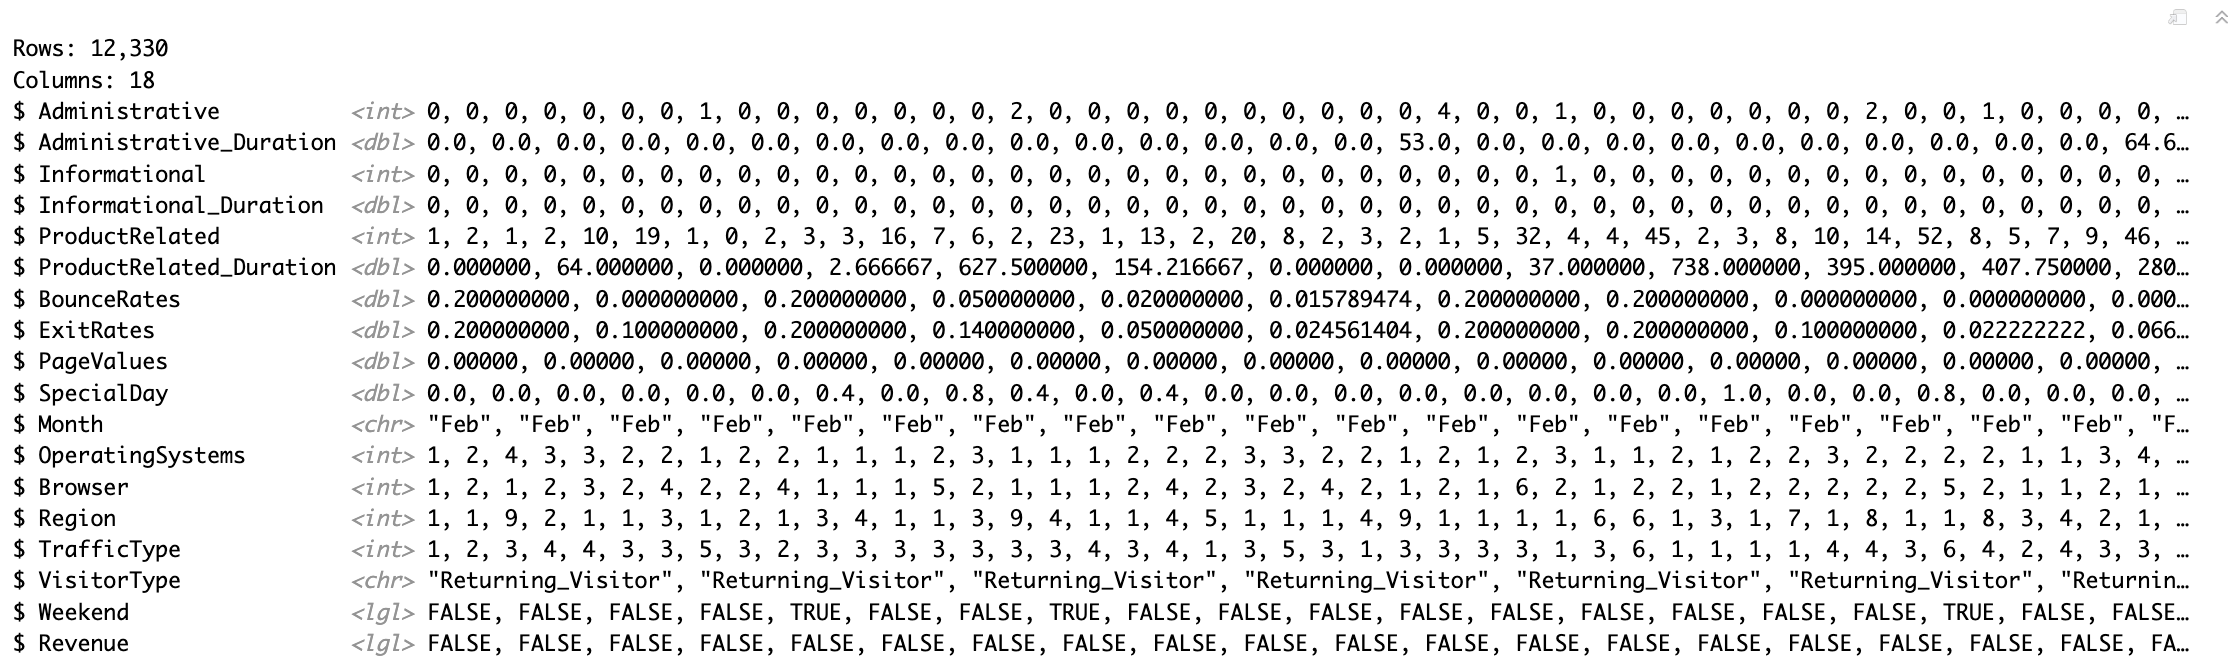
\includegraphics[width=0.5\textwidth]{Screenshot 2024-10-09 at 15.00.28.png}  
    \caption{concise summary of a data }
        \label{fig:example}
   \vspace{0.5cm}
   \end{figure}

   
     
\justifying To guarantee accuracy, column data types were examined and modified throughout data exploration. A check for duplicate rows was also undertaken, with no duplicates detected, protecting data integrity for analysis.
\begin{figure}[h]
    \center
    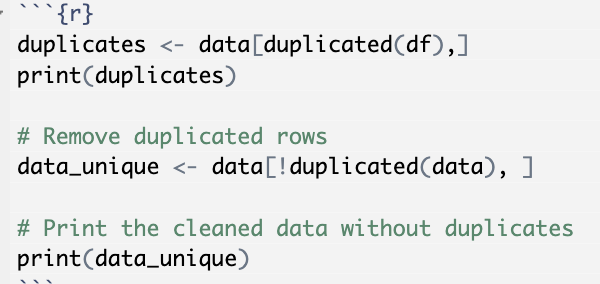
\includegraphics[width=0.5\textwidth]{Screenshot 2024-10-09 at 15.23.25.png}  
    \caption{Checking and removing the duplicate rows}
    \label{fig:example}
    \vspace{0.5cm}
\end{figure}

\subsection{Missing Values}
An extensive search for null values was done first. It was determined through analysis that the dataset included zero null values.
\begin{figure}[h]
    \center
    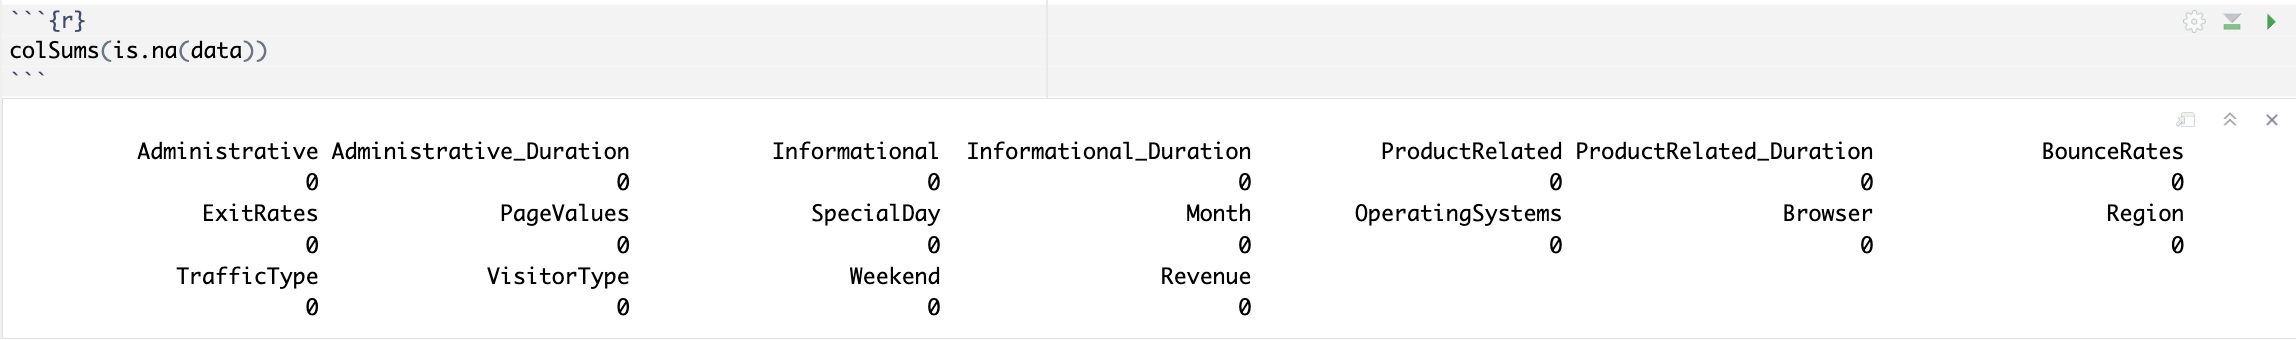
\includegraphics[width=0.5\textwidth]{Screenshot 2024-10-09 at 22.27.50.png}  
    \caption{Checking missing value}
    \label{fig:example}
    \vspace{0.5cm}
\end{figure}

\newpage


\section{Data visualization}
Data visualization makes data easier to grasp by placing it in a visual context and highlighting correlations, patterns, and trends that would be overlooked in text-based data. It converts datasets into graphical formats—often common charts and graphs—that are simpler for the human brain to comprehend (Islam & Jin, 2019) \cite{Islam}.We use a variety of visualization approaches in this part to find patterns, trends, and connections in the data from online shoppers. The idea is to give intuitive insights into consumer behavior by turning raw data into visual representations, which will aid in a better understanding of the variables impacting online purchase decisions.

\textbf{Utilizing ggplot2}: As to Wickham (2016) \cite{Wickham}, ggplot2 makes it easier to create intricate, multi-layered visualizations with a straightforward language, hence streamlining the process of generating beautiful charts. Wickham created the ggplot2 package, a R data visualization tool that produces sophisticated, publication-ready visualizations. In line with Wilkinson's "The Grammar of Graphics," it provides an adaptable interface for assembling various visualizations. Because of its adaptability, simplicity of use, and capacity to generate excellent plots for data analysis, ggplot2 is often utilized.(Xia et al., 2018) \cite{Xia} In a similar vein, interactive visualizations and dashboard are  made with the help of shiny and plotly, which improve user interaction and data exploration.


\subsection{Answering the questions through data visualization}
This part uses the R language, the ggplot2 and plotly packages, to effectively visualize data in order to achieve the above-mentioned aims.

\vspace{0.5cm}

\textbf{User Engagement Analysis} \\

\textbf{1. How does the time spent on different page categories (Administrative, Informational, ProductRelated) correlate with revenue generation? Which pages are most effective at engaging users?} \\[5pt] % Adds 10pt space

The line plot reveals that Returning Visitors exhibit the highest levels of involvement and spend a large amount of time on the site in comparison to New Visitors and Others, according to the analysis of user engagement. December and March have the highest levels of involvement, which is probably due to seasonal marketing or noteworthy occasions. On the other hand, New Visitors' low involvement is constant over the course of every month, indicating the need for better techniques to turn them into more engaged users.


\begin{figure}[h]
    \centering
    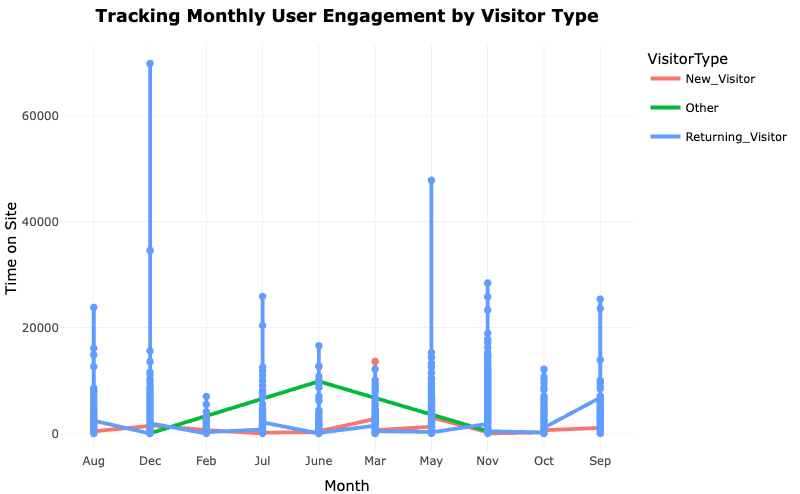
\includegraphics[width=0.82\textwidth]{Trackig monthly user engangement based on month.png}  
    \caption{Tracking Monthly User Engagement by Visitor Type}
\end{figure}

\FloatBarrier
The violin plot shows the distribution of \textit{Time\_on\_Site} for sessions that led to revenue (\textit{Revenue = TRUE}) versus those that did not (\textit{Revenue = FALSE}). Sessions without revenue often had longer times on the site, indicating that spending more time does not necessarily result in purchases. Conversely, sessions with revenue were more clustered, suggesting that purchases were made during shorter, efficient visits. This relates to the effectiveness of different page types—users who efficiently navigate product-related pages are more likely to convert, while excessive time spent, potentially on informational or administrative pages, may not lead to revenue.

\vspace{0.5cm}

\begin{figure}[h]
    \centering
    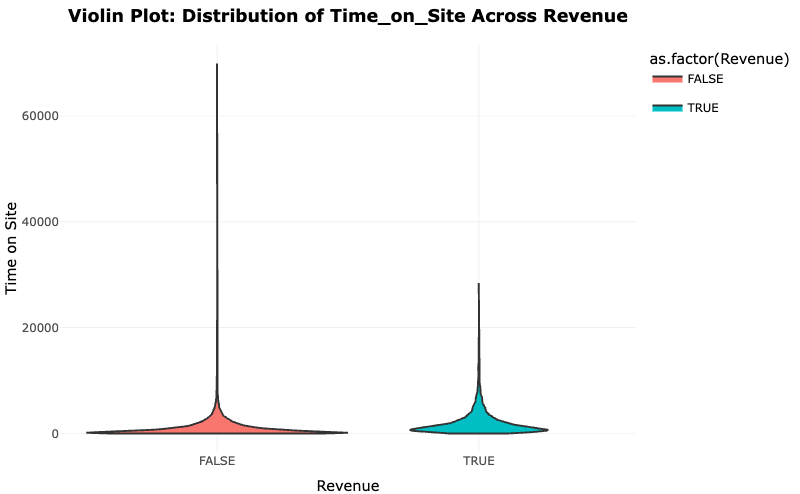
\includegraphics[width=0.82\textwidth]{violin plot distribution of time across site.png}  
    \caption{Violin Plot: Distribution of Time_on_Site Across Revenue}
\end{figure}


\newpage
\textbf{Analyze User Behavior by Demographics}\\

\textbf{1. How does user behavior differ across demographics like Region, OperatingSys-tems, and Browser in terms of revenue generation and engagement? Are there significant variations in user interactions based on these features?} \\[5pt] % 

Depending on the browser a user uses, a bar plot illustrates how different users generate revenue. In comparison to other browsers, users of Browser 2 are far more likely to make revenue, as seen by the plot's noticeable increase. For instance, whereas Browser 1 has a substantial user base, Browser 2 has a far higher conversion rate (or revenue generation), indicating that Browser 2 users are more engaged and inclined to make purchases. A low revenue generation rate for certain browsers, such 3 to 13, may mean that users of particular browsers are less likely to convert or interact with the website less frequently. Plot indicates that the choice of browser clearly affects user behavior and generates income.
\begin{figure}[h]
    \centering
    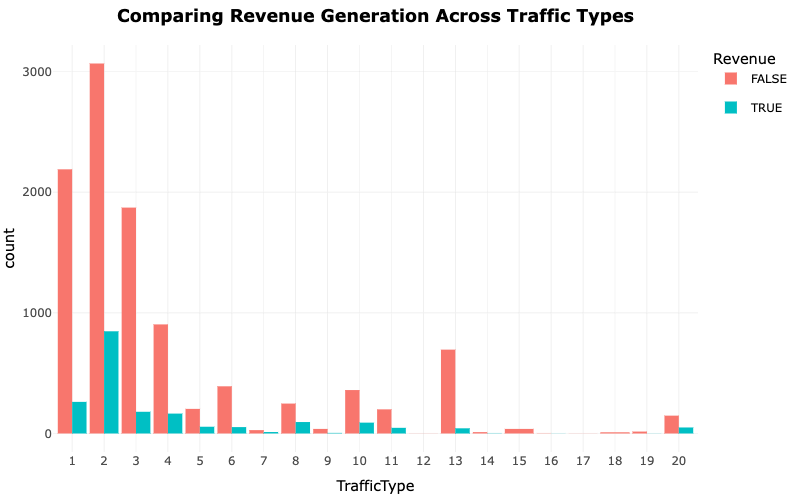
\includegraphics[width=0.82\textwidth]{Revenue Generation Across Browsers.png}  
    \caption{Revenue Distribution Across Different Web Browsers}
\end{figure}

\FloatBarrier
The differences in user behavior between operating systems with regard to income creation are depicted in this graphic. As can be seen, the majority of money is generated by users on Operating System 2, however there are also a respectable number of users on Operating Systems 1 and 3. Though Operating System 1 has a higher percentage of non-revenue-generating users, it still suggests that interaction does not necessarily translate into conversions despite the target audience being greater. With many fewer people earning income from Operating Systems 4 and later, it is evident that certain platforms could not be as effective in encouraging purchases. The plot shows how users' interactions with the website and chance of making purchases can be influenced by their operating system in an effective way.

\begin{figure}[h]
    \centering
    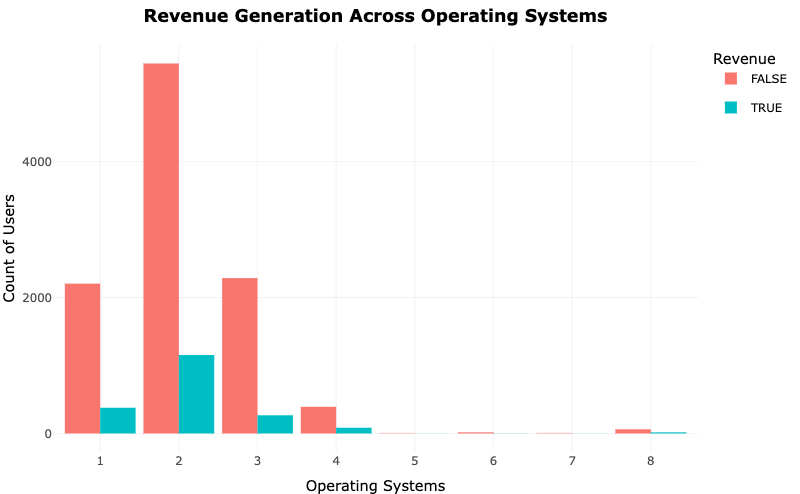
\includegraphics[width=0.82\textwidth]{Revenue Generation Across Operating Systems.png}  
    \caption{Revenue Analysis Across Operating Systems}
\end{figure}
\vspace{0.5cm}

\FloatBarrier
The box plot shows how much time users spend on the website in various geographical areas, broken down by whether or not they brought in money. Region 1 displays a wide range of user time spent on the website, with some users devoting significant amounts of time to the site without necessarily making any money. However, users in Regions 2 and 3 are more productive in terms of making money off the site, even though they spend comparatively less time there. This shows that although certain users may interact with the site more than others, this does not always result in conversions. When paired with income generation, the variations in time spent on the site demonstrate how user involvement (as determined by time on site) differs greatly between areas and can lead to various resultsin terms of revenue.
\begin{figure}[h]
    \centering
    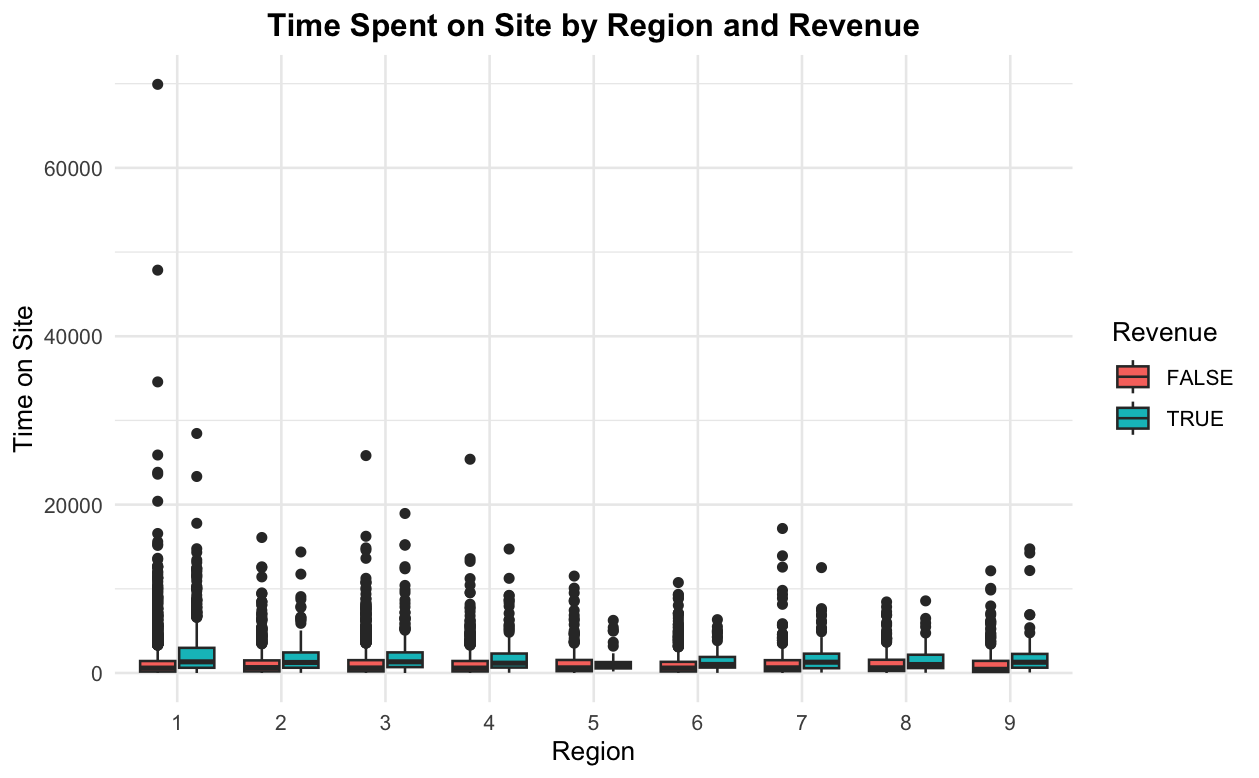
\includegraphics[width=0.82\textwidth]{Time Spent on Site by Region and Revenue.png}  
    \caption{Time Spent on Site by Region and Revenue}
\end{figure}
\vspace{0.5cm}


\FloatBarrier
The disparities in revenue creation between geographic regions are depicted in this bar plot. Although Region 1 has the largest user base, a sizable fraction of its users do not contribute to revenue, suggesting that there may be a problem with engagement or conversion. However, although though Region 2 has fewer users overall, it has a greater percentage of users who generate income, which makes it a more effective region in terms of conversions. Similar trends can be seen in Region 3, where a smaller user base yields comparatively more revenue. This figure illustrates how user behavior is influenced by location, demonstrating how various regions contribute to income in unique ways and how certain places are more conducive to conversions than others.

\begin{figure}[h]
    \centering
    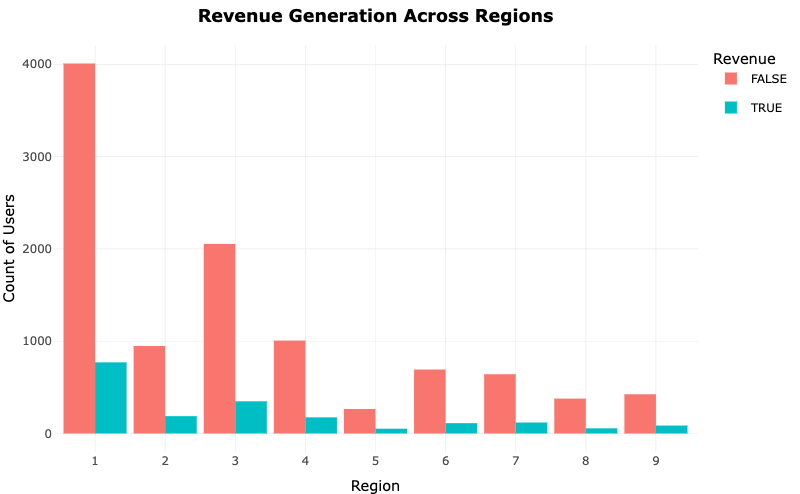
\includegraphics[width=0.82\textwidth]{Revenue Generation Across Regions.png}  
    \caption{Revenue Generation Across Regions}
\end{figure}
\vspace{0.5cm}

\newpage

\textbf{Evaluate the Impact of Visitor Types and Special Events on Revenue}\\

\textbf{1. What is the impact of being a New Visitor versus a Returning Visitor on revenue generation, especially during significant holidays or special days? Are returning visitors more likely to generate revenue during special events?} \\[5pt] % 

An overview of the Visitor Type distribution within the dataset is given by this graph. It demonstrates that Returning Visitors account for a large portion of sessions, far outnumbering both New Visitors and the Other group. This substantial user base of Returning Visitors supports the idea that they are a major source of revenue for the platform and is suggestive of high levels of customer loyalty. In addition to reflecting their lower level of involvement with the site overall, the modest number of New Visitors relative to Returning Visitors is further supported by their negligible revenue-generating contribution.
\begin{figure}[h]
    \centering
    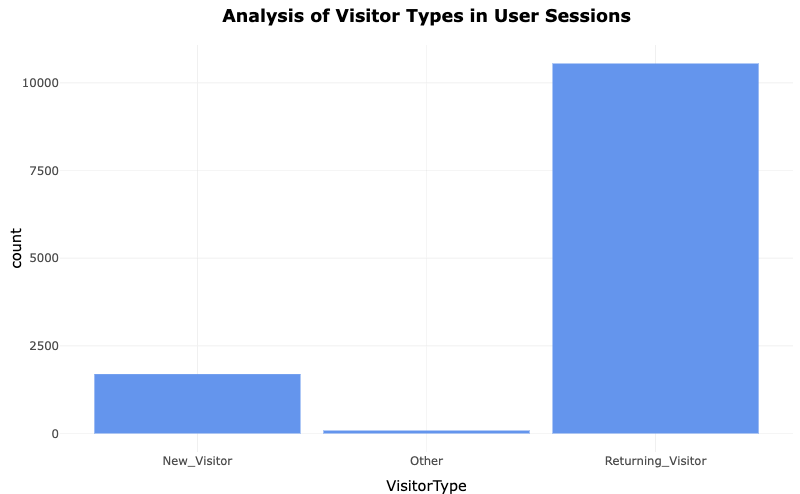
\includegraphics[width=0.82\textwidth]{Analysis of Visitor Types in User Sessions.png}  
    \caption{Analysis of Visitor Types in User Sessions}
\end{figure}
\vspace{0.5cm}

\FloatBarrier
The total revenue generated by new and returning visitors is directly compared in this bar plot. The high number of Returning Visitors who generate revenue (shown in blue) makes it clear that they account for a far higher portion of the total revenue. Even if they are present in large numbers, new visitors are much less likely to bring in money, which emphasizes how crucial it is to keep customers. This shows that, regardless of when they come, Returning Visitors are more likely to make repeat purchases and are more at ease using the platform (perhaps as a result of prior pleasant encounters).

\begin{figure}[h]
    \centering
    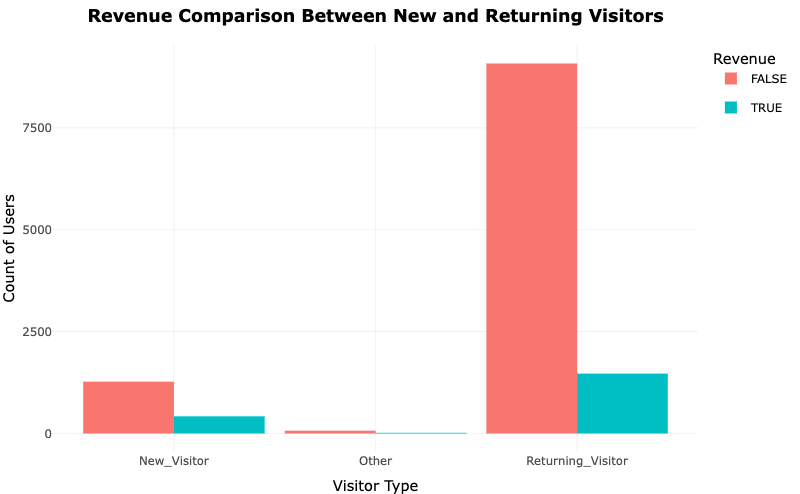
\includegraphics[width=0.82\textwidth]{Revenue Comparison Between New and Returning Visitors.png}  
    \caption{Revenue Comparison Between New and Returning Visitors}
\end{figure}
\vspace{0.5cm}


\FloatBarrier
This graph looks at the differences in income creation between New Visitors, Returning Visitors, and Other Visitors while accounting for the weekend nature of the session. Plotting shows that, on any given day of the week, Returning Visitors generate substantially more revenue than New Visitors. Both weekend and non-weekend sessions exhibit increased income contribution and engagement from Returning Visitors. Conversely, less revenue-generating sessions are had by New Visitors, and their interaction patterns remain the same throughout both weekend and non-weekend sessions. This implies that Weekends have a limited additional influence on the behavior of New Visitors, whereas Returning Visitors are constantly significant for revenue.
\begin{figure}[h]
    \centering
    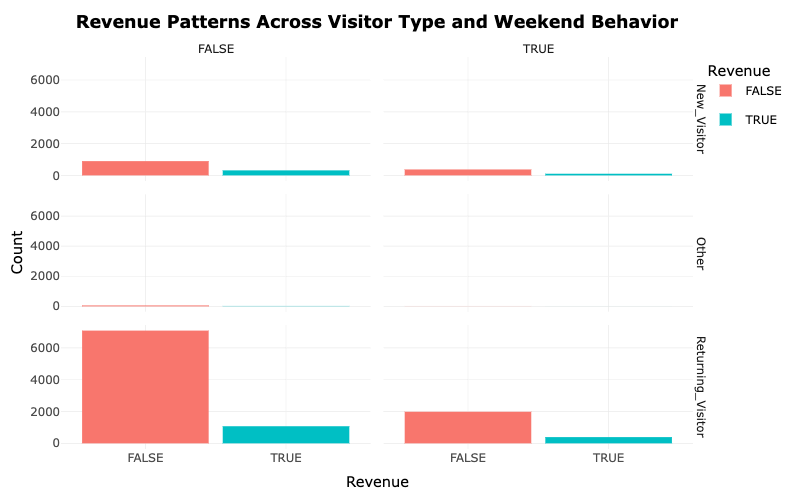
\includegraphics[width=0.82\textwidth]{Revenue Patterns Across Visitor Type and Weekend Behavior.png}  
    \caption{Revenue Patterns Across Visitor Type and Weekend Behavior}
\end{figure}
\vspace{0.5cm}

In a nutshell Regardless of the session schedule (weekends or weekdays) or closeness to special events, it is evident from all three plots that Returning Visitors are essential to generating money. The larger number of sessions from Returning Visitors and their better conversion rate demonstrate how important it is for the platform to maintain income streams from customer retention. The likelihood of income generation from new visitors is significantly lower. This implies that, although attracting new users is vital, retaining and involving existing users is more critical to optimize revenue, particularly on vacations or special occasions.
\vspace{0.5cm}


\textbf{Understand the Effects of Bounce and Exit Rates}\\

\textbf{1. What is the effect of high BounceRates and ExitRates on different regions in terms of revenue generation? Are there specific regions with high bounce or exit rates that require improvements in content or design?} \\[5pt] % 

The relationship between BounceRates and ExitRates is depicted in this aspect scatter plot, which allows for the distinction between sessions that generate income (True) and those that do not (False). Higher BounceRates are closely correlated with higher ExitRates for sessions without revenue (False), suggesting that users frequently exit the site without purchasing, most likely as a result of discontent or lack of engagement. Revenue-generating sessions, on the other hand, show significantly lower BounceRates and ExitRates, indicating a higher likelihood of purchases from visitors who stay on the site longer and see more pages. This demonstrates how revenue creation is adversely affected by high bounce and exit rates, and how improving these factors may improve user retention and increase conversions.
\begin{figure}[h]
    \centering
    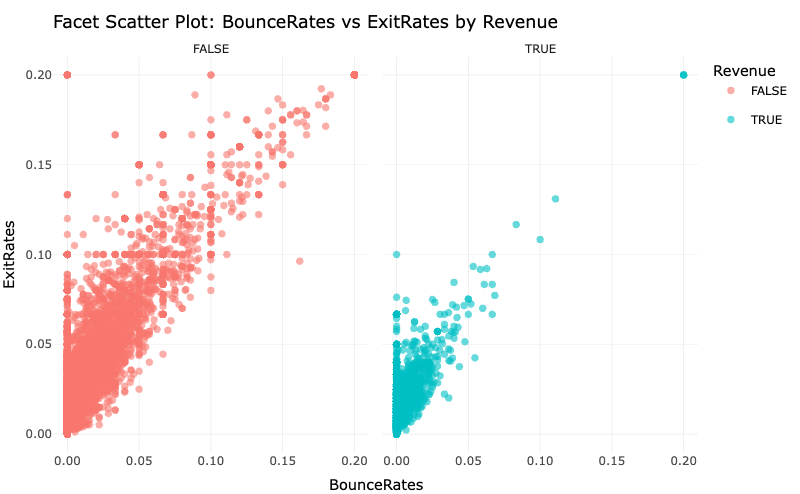
\includegraphics[width=0.82\textwidth]{Facet Scatter Plot- BounceRates vs ExitRates by Revenue.png}  
    \caption{Analyzing Bounce Rates vs. Exit Rates by Revenue Segments}
\end{figure}
\vspace{0.5cm}

\FloatBarrier
The relationship between BounceRates and ExitRates is shown in this bubble chart, where the sizes of the bubbles indicate various areas. Whether or not the session generated revenue is indicated by the color coding (True or False). Since most of the bubbles in the high BounceRate/ExitRate section are red, it is evident that a high concentration of red bubbles, which reflect sessions that do not generate money, tend to correspond with lower revenue. Given their significant contribution to non-revenue sessions, the regions with higher BounceRates and ExitRates require attention. The few blue bubbles, which stand for sessions that generate income, are situated in regions with lower exit and bounce rates, indicating that lowering these rates may have the effect of raising revenue creation.
\begin{figure}[h]
    \centering
    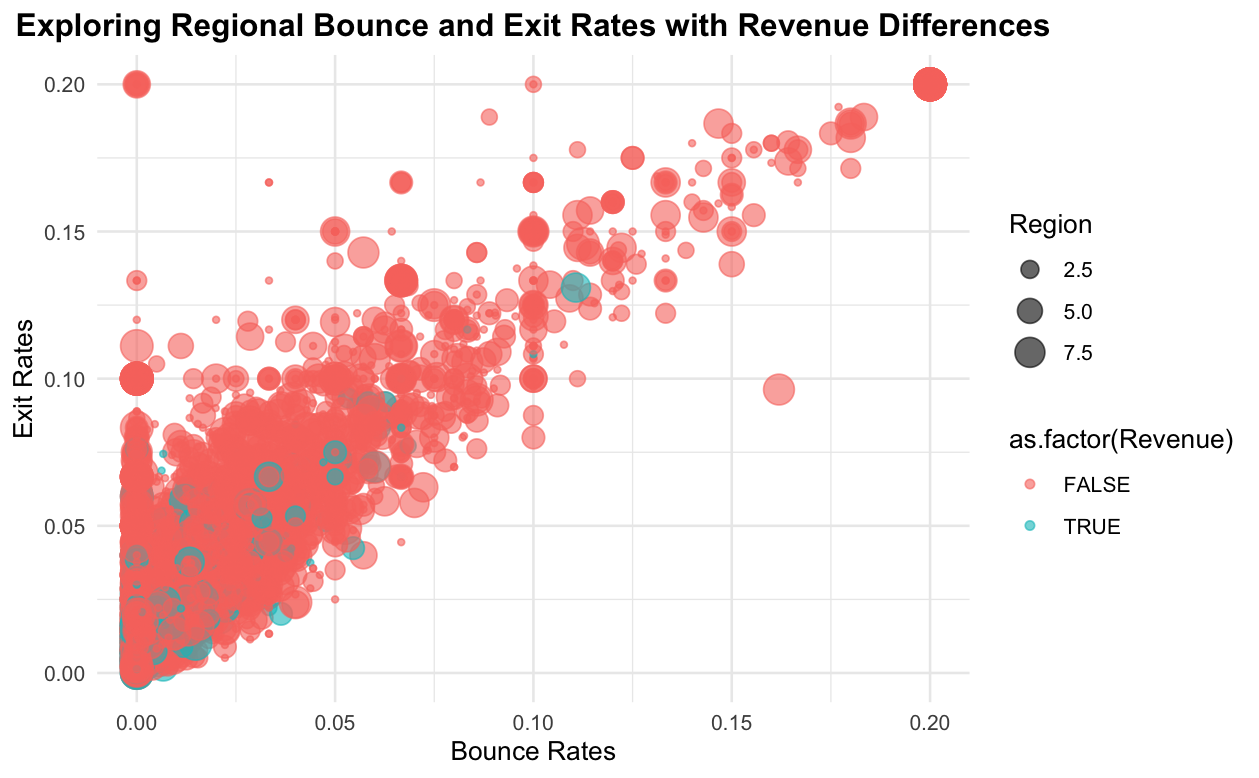
\includegraphics[width=0.82\textwidth]{Exploring Regional Bounce and Exit Rates with Revenue Differences.png}  
    \caption{Exploring Regional Bounce and Exit Rates with Revenue Differences}
\end{figure}
\vspace{0.5cm}

From the charts it is clear that High BounceRates and ExitRates have a negative effect on income creation, as both plots highlight. It appears that in order to retain users and lower early exits, content or site design upgrades are necessary, as the regions and sessions with higher BounceRates and ExitRates predominantly lead to non-revenue-generating sessions. Improved user engagement is crucial for driving up sales, as seen by the constant correlation between lower bounce rates and exit rates and revenue creation.

\FloatBarrier
From this time series plot depicting bounce rates across different months, several insights can be derived. The chart shows that bounce rates consistently fluctuate throughout the months, with notable peaks reaching up to 0.20, indicating a high proportion of users leaving after visiting only a single page. Specifically, in months like December, February, and November, bounce rates appear higher compared to others, suggesting that during these months, user engagement may be weaker. This could be attributed to seasonal factors or ineffective content that doesn't captivate visitors enough to explore further.


The line patterns also demonstrate that some months—like May and September—separately saw abrupt declines in bounce rates. These times may be associated with campaigns that were effective, increased user interaction, or site optimizations that decreased bounce rates and increased user interaction.


In general, the results show that in order to keep visitors engaged during the months with higher bounce rates, specific tactics are required, such as enhancing page content or user experience. On the other hand, months with lower bounce rates can indicate times when the site's campaigns or content are running smoothly, potentially offering best practices to follow in subsequent months. Periods during which the website might further enhance its efforts to retain users can be identified thanks to this time-series analysis.
\begin{figure}[h]
    \centering
    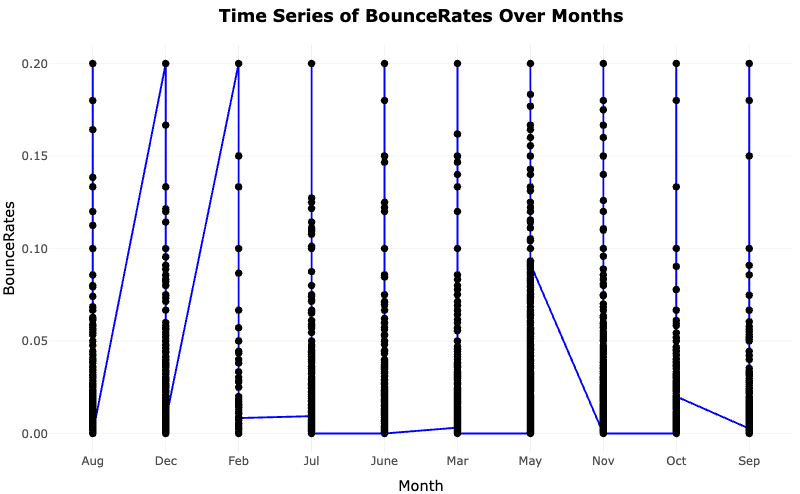
\includegraphics[width=0.82\textwidth]{Time Series of BounceRates Over Months.png}  
    \caption{Time Series of BounceRates Over Months}
\end{figure}
\vspace{0.5cm}

\newpage




\vspace{0.5cm}


\textbf{Investigate Conversion Funnel Effectiveness}\\

\textbf{1. How effective are different traffic sources in leading to successful conversions? At what points in the user journey are users most likely to drop off, and how does this affect the overall conversion rate?} \\[5pt] % 


The distribution of traffic sources is depicted in this plot, with TrafficTypes 1, 2, and 5 accounting for the majority of visits—TrafficType 1 in particular, reaching close to 4000 visits. Numerous other forms of traffic, however, result in far less traffic. The fact that a small number of sources predominate suggests that efforts should be directed toward optimizing the top traffic kinds while investigating methods to enhance the performance of lower-contributing channels in order to diversify the traffic base.
\begin{figure}[h]
    \centering
    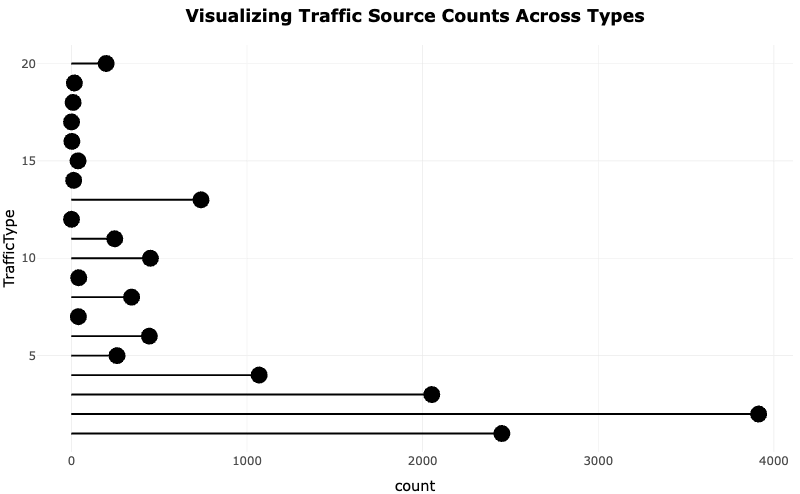
\includegraphics[width=0.82\textwidth]{Visualizing Traffic Source Counts Across Types.png}  
    \caption{Visualizing Traffic Source Counts Across Types}
\end{figure}
\vspace{0.5cm}


\FloatBarrier
For every traffic kind, the number of revenue-generating sessions is plotted on a line throughout several months. Certain traffic types appear to be especially effective during peak shopping seasons, as evidenced by the noticeable jump in conversions that some traffic sources, such as Traffic Type 2, exhibit during particular months (e.g., November). While some traffic categories show steady but reduced effectiveness over the course of the year, others remain relatively level in terms of conversion performance. This graph aids in determining which traffic sources are more productive at particular periods of the year and can direct marketing efforts toward enhancing underperforming sources in months with low conversion rates.
\begin{figure}[h]
    \centering
    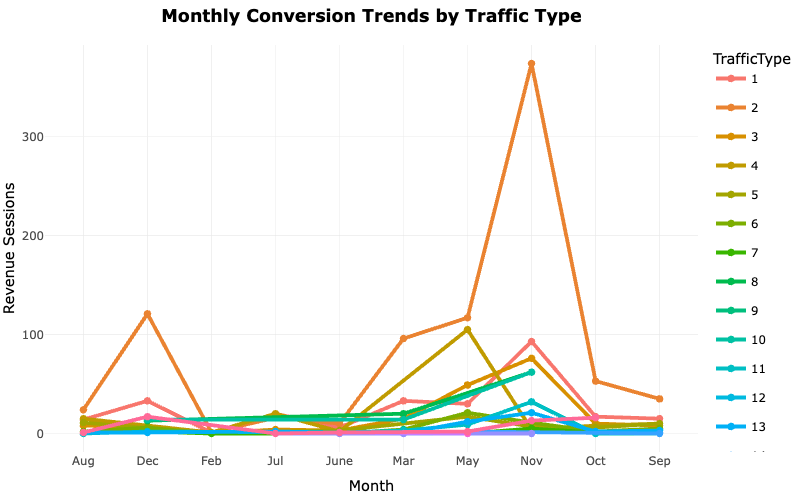
\includegraphics[width=0.82\textwidth]{Monthly Conversion Trends by Traffic Type.png}  
    \caption{Monthly Conversion Trends by Traffic Type}
\end{figure}
\vspace{0.5cm}

\FloatBarrier
The treemap shows how various traffic sources contribute to total revenue in a visual manner. When compared to other traffic sources, such Traffic Types 15 and 18, which are smaller and so indicate less conversions, traffic sources like 2, 3, and 1 have the largest regions and hence contribute the most to income. With the help of this treemap, we can quickly determine which traffic sources convert well and which ones may require improvement. Prioritizing which sources to concentrate on can assist increase the conversion rate overall.
\begin{figure}[h]
    \centering
    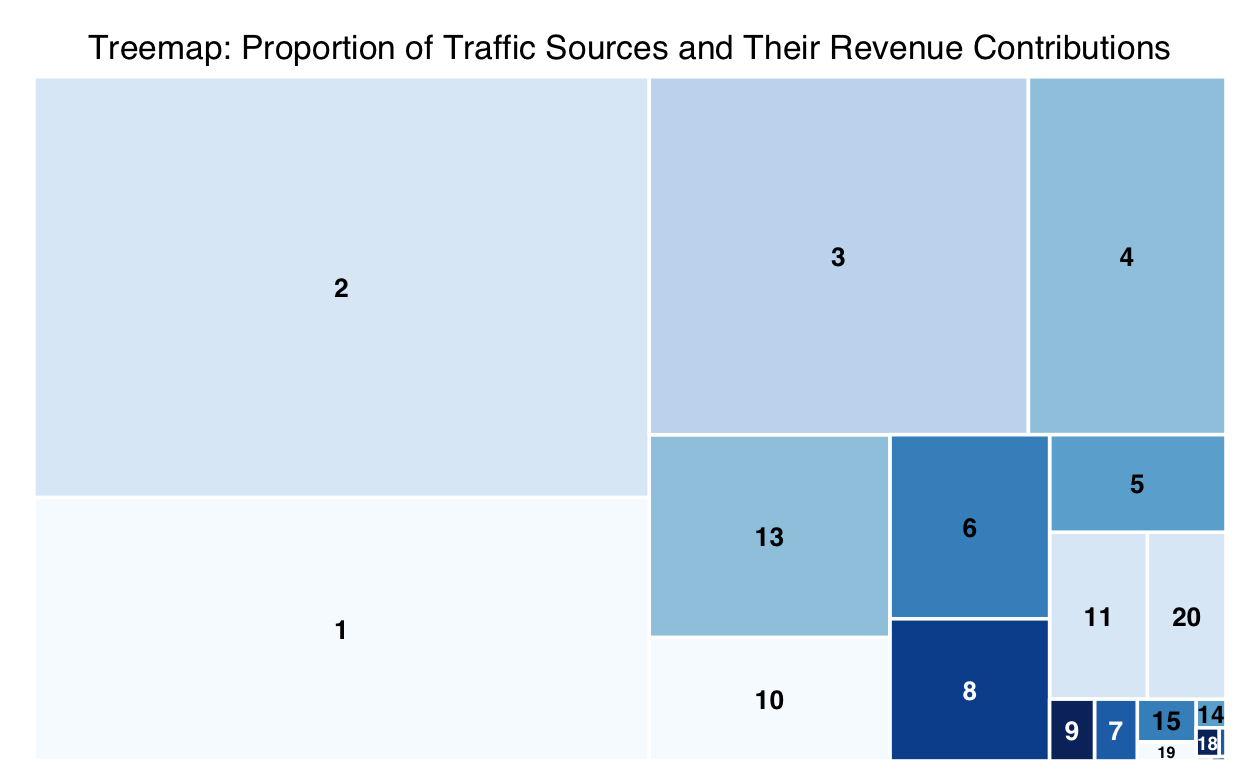
\includegraphics[width=0.82\textwidth]{Proportion of Traffic Sources and Their Revenue Contributions.png}  
    \caption{Proportion of Traffic Sources and Their Revenue Contributions}
\end{figure}
\vspace{0.5cm}


\FloatBarrier
The efficacy of various traffic sources (TrafficTypes) in producing revenue sessions is shown in the bar chart titled "FConversion from Traffic Type to Revenue Sessions". Among the traffic types, Types 1, 2, and 3 are the most successful in converting visitors into paying customers, as they accounted for the greatest number of sessions. With almost 4000 revenue sessions, Traffic Type 1 produced the most, followed by Traffic Types 2 and 3 (847 and 262 sessions, respectively). Conversely, traffic types 14, 15, and 19 showed a significant drop-off rate, contributing nearly no revenue sessions or none at all.This graph shows that whereas certain traffic sources are quite successful at generating conversions, others are not so successful, indicating that consumers who come from these underperforming traffic sources are more likely to abandon their journey early. The information gleaned from this plot can direct content modifications or low-performing source targeting tactics to enhance the overall
\begin{figure}[h]
    \centering
   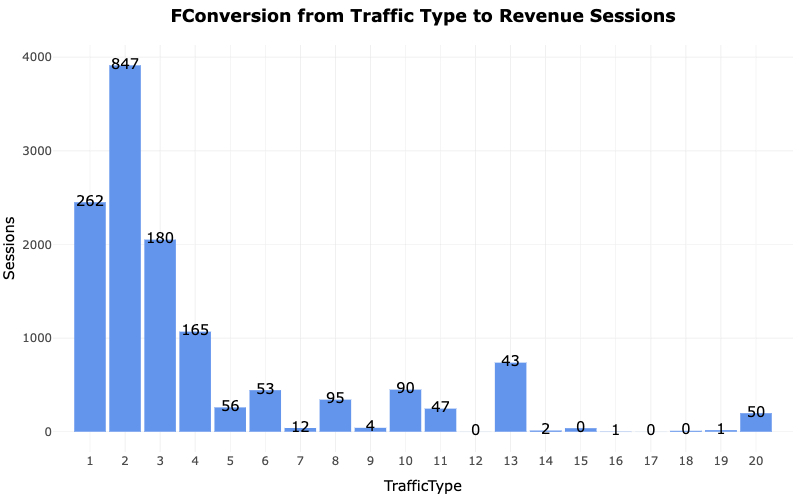
\includegraphics[width=0.82\textwidth]{FCOn.png}  
    \caption{Conversion from Traffic Type to Revenue Sessions}
\end{figure}
\vspace{0.5cm}

\FloatBarrier
This bar graph contrasts, for each traffic source, the number of sessions that brought in money (blue bars) with those that did not (red bars). We observe that traffic categories 1, 2, and 3 provide a lot of sessions, yet a big percentage of those sessions don't result in income. There appears to be a large number of users quitting after coming from these sources of traffic, based on the disparity between the revenue and non-revenue sessions. Particularly, Traffic Type 2 produces the greatest number of sessions but has a large percentage of non-revenue sessions, suggesting that there is potential to optimize the conversion of these consumers. This chart is essential for figuring out where visitors are likely to lose interest and leave the website without making a purchase.
\begin{figure}[h]
    \centering
    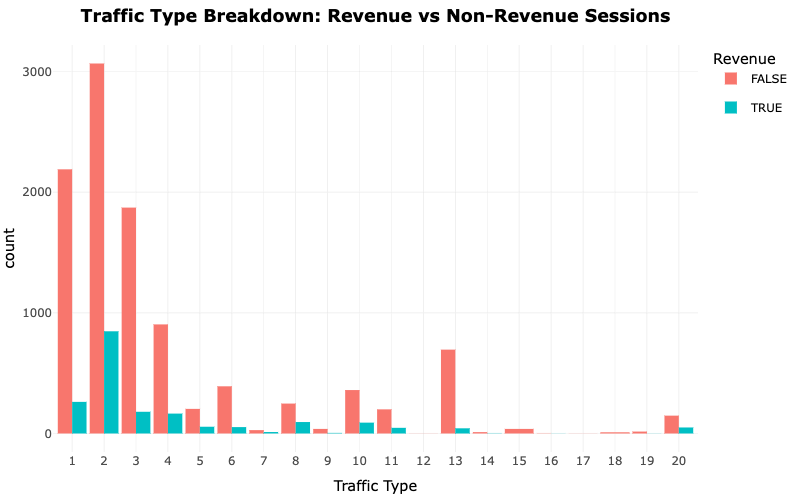
\includegraphics[width=0.82\textwidth]{Traffic Type Breakdown- Revenue vs Non-Revenue Sessions.png}  
    \caption{Traffic Type Breakdown- Revenue vs Non-Revenue Sessions}
\end{figure}
\vspace{0.5cm}

\FloatBarrier
All in all, the plots show that although Traffic Types 1, 2, and 3 are the most successful at resulting in successful conversions, there are still drop-offs that impact the conversion rate as a whole. Significant drop-off points in the user journey are indicated by the extremely poor conversion rates of other traffic sources, especially Types 14, 15, and 16. To increase the overall conversion rate, these visualizations advise concentrating on enhancing the user experience or more precisely directing traffic from various sources.
\vspace{0.5cm}

\textbf{Feature Correlation}\\

\textbf{1. What relationships exist between numeric features (e.g., ProductRelated Duration,PageValues) and revenue outcomes? Which features are strong predictors of user behavior?} \\[5pt] % 

The relationships between various numerical variables and how they affect user behavior and revenue consequences are revealed by the correlation matrix graphic. A weak negative correlation (-0.185) has been observed between ProductRelated\_Duration and BounceRates. This suggests that users who spend longer time on product-related pages are somewhat less likely to bounce, which could indicate a potential interest in making a purchase. The relatively slight positive association (0.053) found with PageValues, however, suggests that revenue creation is not considerably impacted by the amount of time spent on product pages. Higher page values generally tend to modestly lower bounce rates, increasing users' likelihood to stay and continue browsing, according to the weak negative correlation between PageValues and BounceRates (-0.119). Additionally, PageValues have poor correlations with other features, such as ProductRelated\_Duration, Informational\_Duration, and Administrative\_Duration, indicating a greater degree of correlation with factors impacting purchase behavior rather than the amount of time spent on different sorts of pages. The data indicates that there is a weak negative correlation between BounceRates and almost all other features, such as ProductRelated\_Duration, Administrative\_Duration (-0.144), and Informational\_Duration (-0.074). This suggests that users who interact more with the website's various sections are somewhat less likely to bounce. The data indicates that there is a moderate positive correlation between Administrative\_Duration and Informational\_Duration (0.238). This suggests that users who spend time on administrative pages also interact with informational pages, which is indicative of overall site engagement. Likewise, there is a moderate connection (0.355) between Administrative\_Duration and ProductRelated\_Duration, suggesting that individuals who are involved in administrative chores are also likely to visit pages connected to products. A moderate correlation (0.347) has been found between Informational\_Duration and ProductRelated\_Duration, indicating that users who engage with informational content also tend to interact with product pages, which is consistent with a wider pattern of site usage. To summarize, neither revenue nor user behavior can be significantly predicted by a single characteristic; nonetheless, there are some indications of revenue and engagement from the weak correlations between ProductRelated\_Duration and BounceRates, as well as between PageValues and other variables.
\begin{figure}[h]
    \centering
    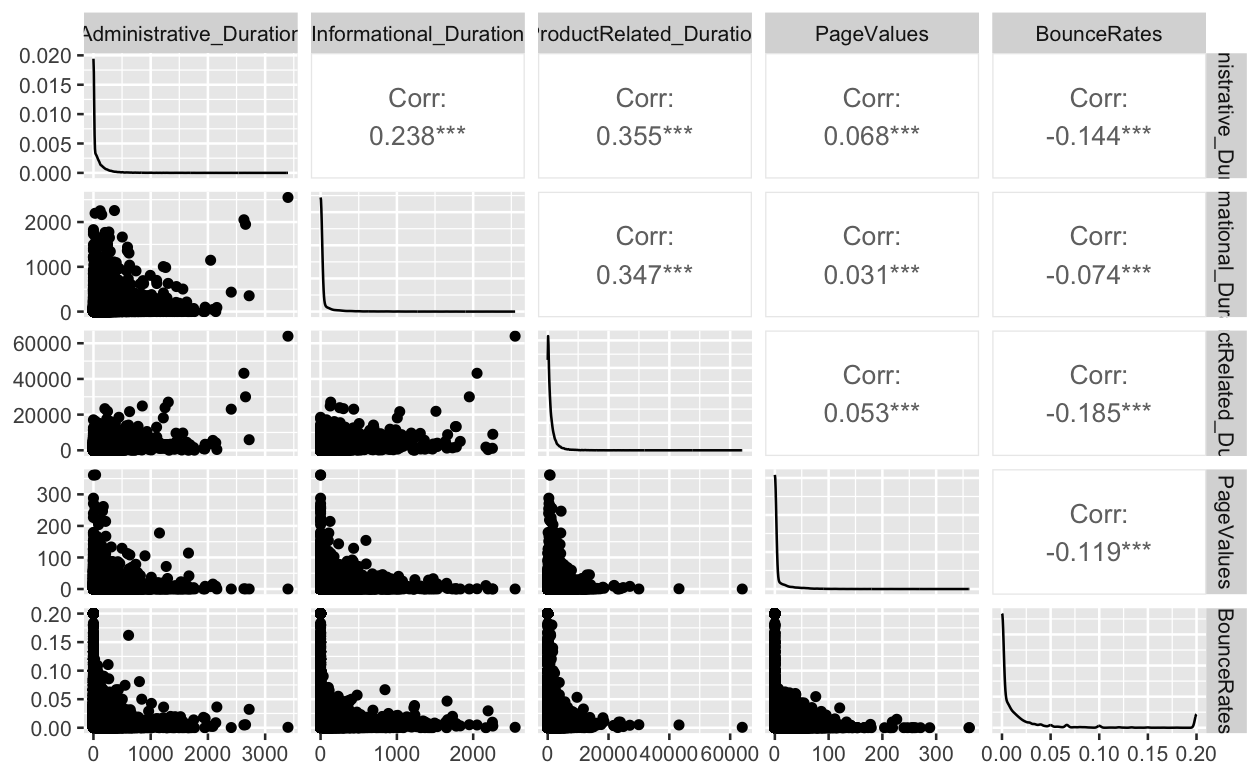
\includegraphics[width=0.82\textwidth]{Correlation.png}  
    \caption{Traffic Type Breakdown- Revenue vs Non-Revenue Sessions}
\end{figure}
\vspace{0.5cm}

\newpage

\textbf{Revenue Distribution}\\

\textbf{1. How is the distribution of PageValues across revenue categories? What insights can be drawn about prioritizing high-value content?} \\[5pt] % 

The distribution of PageValues shows that most pages have values that are almost equal to zero, which suggests that most pages visited during sessions don't make a big difference in terms of making money. There are, nevertheless, a select few high-value pages that are essential in encouraging customers to finish purchases. Despite being uncommon, these pages are the main sources of income. Concentrating on these high-value pages is crucial for content prioritization since they have a direct impact on conversions. Through optimization and enhancement of these pages, companies can greatly boost sales. The distribution's long tail indicates that a small percentage of pages account for the majority of the value, emphasizing the significance of improving those pages to optimize their influence. Thus, focusing attention on high-value pages can result in significant improvements in revenue creation even when the majority of content may not directly drive sales. 
\begin{figure}[h]
    \centering
    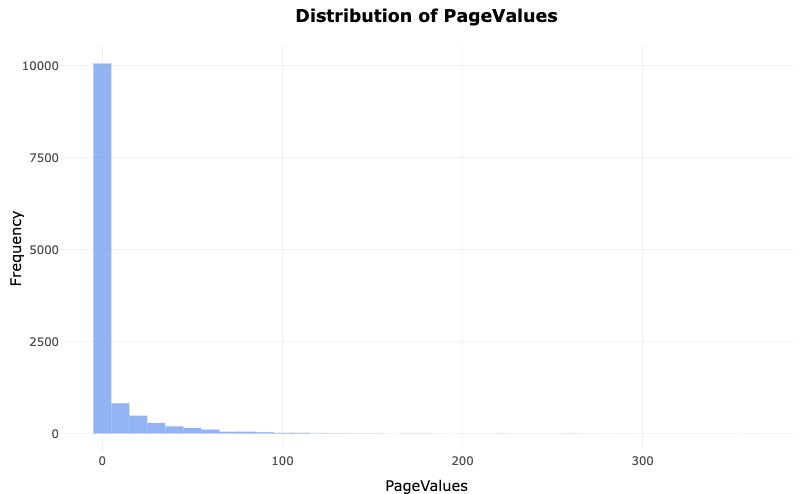
\includegraphics[width=0.82\textwidth]{Distribution of PageValues.png}  
    \caption{Distribution of PageValues}
\end{figure}
\vspace{0.5cm}

\FloatBarrier
The graph shows the link, broken down by whether a session generated income, between ProductRelated\_Duration (the amount of time spent on product-related pages) and PageValues (the contribution of a page to revenue creation). The PageValue distribution indicates that even with shorter durations on product-related pages, sessions that result in revenue typically have higher PageValues. Conversely, the majority of non-revenue-generating sessions have lower PageValues, suggesting that even in cases when the PageValue is low, longer interaction periods may not be associated with successful transactions.

This emphasizes how crucial it is to concentrate on high-quality content. Regardless of the amount of time consumers spend on a page, those with greater PageValues are considerably more effective in generating revenue. Thus, it is better to focus on improving high-value pages rather than just spending more time on product pages. The figure implies that even in shorter sessions, people might be persuaded to convert rapidly if they interact with highly optimized, valuable information. This highlights the necessity of having such powerful content on the website easily accessible.

\begin{figure}[h]
    \centering
    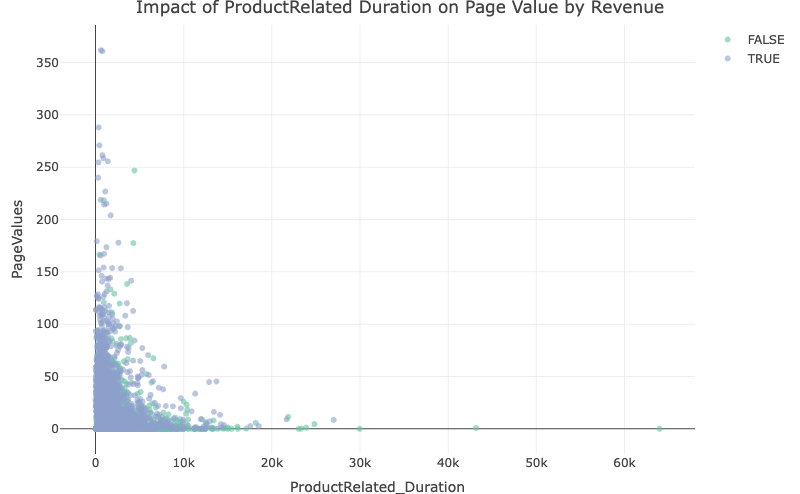
\includegraphics[width=0.82\textwidth]{Impact of ProductRelated Duration on Page Value by Revenue.png}  
    \caption{Impact of ProductRelated Duration on Page Value by Revenue}
\end{figure}
\vspace{0.5cm}

\FloatBarrier
As a result, the plot emphasizes the need of giving high-value content top priority by showing a direct correlation between increased PageValues and income production. Through optimization of pages that are important drivers of transactions, organizations can increase revenue and conversions without increasing user engagement.
\vspace{0.5cm}


\textbf{Cohort Analysis:}\\

\textbf{1. How do new and returning visitors contribute to revenue generation over time? What insights does this provide into customer loyalty and retention strategies?} \\[5pt] % 

A pie chart that displays the percentage of each type of visitor to the website reveals that, of all sessions, 85.6\% are from repeat visitors, 13.7\% are from new visitors, and only 0.68\% are from the "Other" category. The overwhelming presence of repeat visitors in website traffic is indicated by this statistics, which implies that these users are more involved with the platform. The substantial number of repeat visitors highlights the significance of client retention tactics. Businesses can profit from the majority of their traffic, which originates from this recurring client base, by concentrating on retaining current consumers.
\begin{figure}[h]
    \centering
    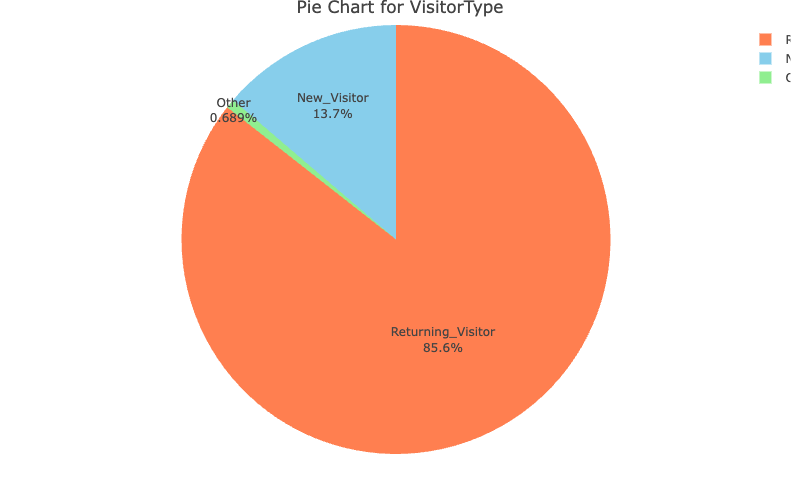
\includegraphics[width=0.82\textwidth]{Pie Chart for VisitorType.png}  
    \caption{Pie Chart for VisitorType}
\end{figure}
\vspace{0.5cm}

\FloatBarrier
This line graph shows the total amount of money made over a period of many months from various visitor kinds. Plotting makes it abundantly evident that, compared to new or other sorts of visitors, repeat visitors significantly increase sum revenue. Travelers returning from previous visits provide for the majority of revenue rises during peak months, especially May, July, and November; new tourists make up very little of the total. It suggests that businesses should place a high priority on preserving and growing connections with these devoted consumers, as evidenced by the fact that returning visitors are not only frequent users but also the primary source of income.
\begin{figure}[h]
    \centering
    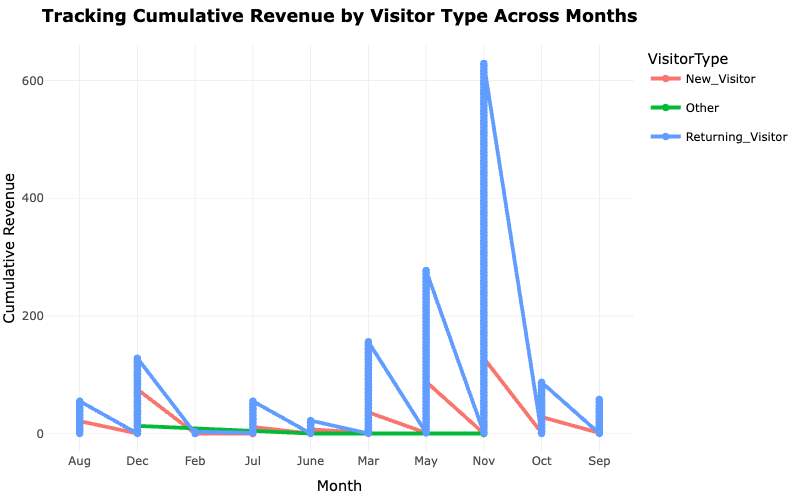
\includegraphics[width=0.82\textwidth]{Tracking Cumulative Revenue by Visitor Type Across Months.png}  
    \caption{Tracking Cumulative Revenue by Visitor Type Across Months}
\end{figure}
\vspace{0.5cm}
\newpage

\FloatBarrier

The revenue production by kind of visitor is visualized via cohort analysis over time, demonstrating that higher revenue is consistently generated by returning visitors, especially in May, June, and November. On the other hand, most of the sessions of new visitors do not result in purchases, and so contribute less to revenue overall. Given that returning visitors are more likely to complete transactions, this disparity between visitor types highlights the value of concentrating on client loyalty. To increase long-term revenue production, strategies to turn new visitors into loyal clients should be given priority.
\begin{figure}[h]
    \centering
    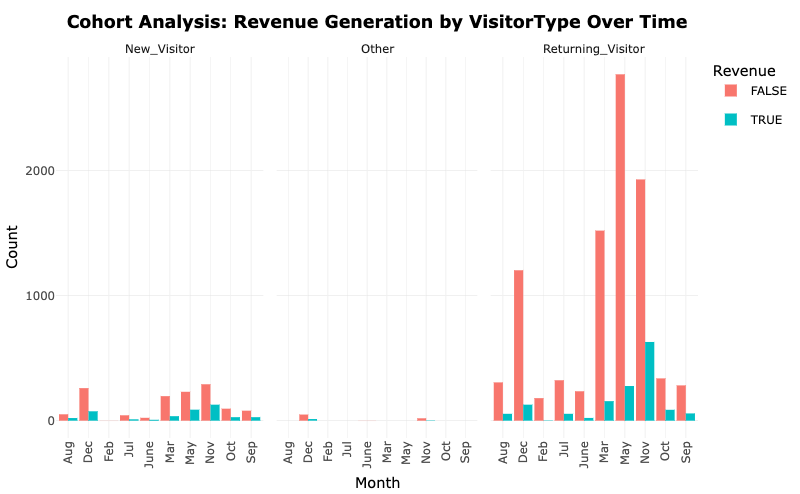
\includegraphics[width=0.82\textwidth]{Cohort Analysis- Revenue Generation by VisitorType Over Time.png}  
    \caption{Cohort Analysis- Revenue Generation by VisitorType Over Time}
\end{figure}
\vspace{0.5cm}

\FloatBarrier
Together, these three plots show that repeat customers are the main source of income, highlighting the significance of loyalty and retention programs. Programs designed to draw in and keep repeat business are probably going to provide the best results. On the other hand, considering that they make up a smaller portion of initial revenue generating, techniques to turn visitors into devoted patrons are crucial for sustained expansion.
\vspace{0.5cm}


\textbf{Geographic Analysis:}\\

\textbf{1. How does revenue generation differ by geographic region? What markets show the most potential for growth?} \\[5pt] % 

\FloatBarrier

By showing the percentage of sessions that ended in a purchase, the graphic demonstrates how income production differs between different locations. Higher revenue-rate regions—1, 2, 5, and 9—indicate that they are high-performing marketplaces because they clearly contribute to the site's total revenue. On the other hand, areas like 3, 6, and 8 have lower revenue rates and offer room for expansion even with their possible high traffic. To increase conversion rates, these underperforming areas could profit from localized advertising, improved user engagement, or focused marketing techniques. Businesses can increase total revenue and broaden their market reach by identifying these untapped potential areas and concentrating on tactics to improve their performance. Strategic decision-making for regional growth is aided by the insightful information this study offers on geographic performance.
\begin{figure}[h]
    \centering
    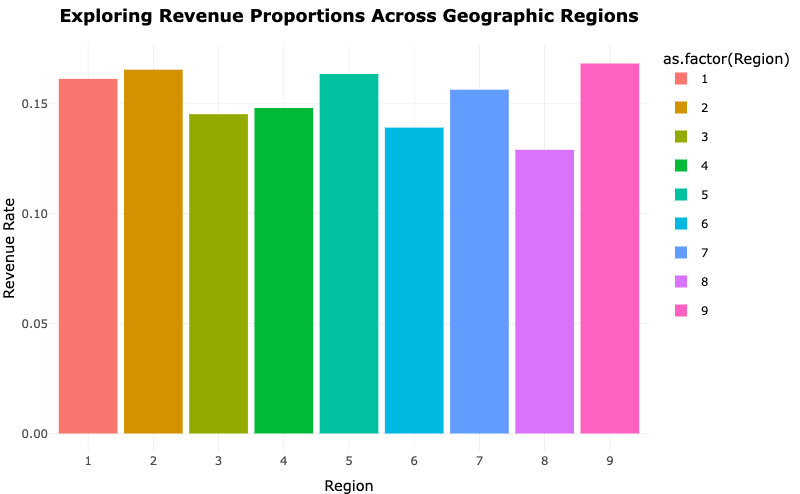
\includegraphics[width=0.82\textwidth]{Exploring Revenue Proportions Across Geographic Regions.png}  
    \caption{Exploring Revenue Proportions Across Geographic Regions}
\end{figure}
\vspace{0.5cm}


\textbf{Visitor Type and Revenue Generation Insights:}\\

\textbf{1. How does revenue generation differ between Returning Visitors and New Visitors across various months? What strategies can be implemented to enhance engagement and conversions among new visitors?} \\[5pt] % 

\FloatBarrier

Regarding the ways in which Returning Visitors, New Visitors, and Others contribute to income production over time, the heatmap provides various important insights. The most notable conclusion is that Returning Visitors are the main sources of money, continuously making a substantial contribution all year long, particularly in November and May when revenue peaks are easily observed. This highlights the significance of client retention initiatives by indicating that repeat consumers are highly engaged and inclined to make more purchases. Revenue creation is significantly influenced by seasonal trends as well. November is notable because of probable events like Cyber Monday and Black Friday, while May also exhibits a notable rise. Based on these statistics, firms should launch targeted advertisements during certain months to increase sales.

Conversely, the heatmap's lighter color representation of New Visitors indicates that they make up a smaller portion of total income. This indicates the need for better onboarding procedures or focused engagement methods, as it implies that new visitors might need more time or interaction before becoming paying clients. In all months, the Other Visitors category generates very little income, suggesting that this group has very little effect on revenue and that more research may be necessary to better understand their behavior or to focus marketing efforts. The heatmap, taken as a whole, emphasizes the vital significance of repeat visitors, the effect of seasonality on income, and the potential for raising conversion rates among new and other visitor categories.
\begin{figure}[h]
    \centering
    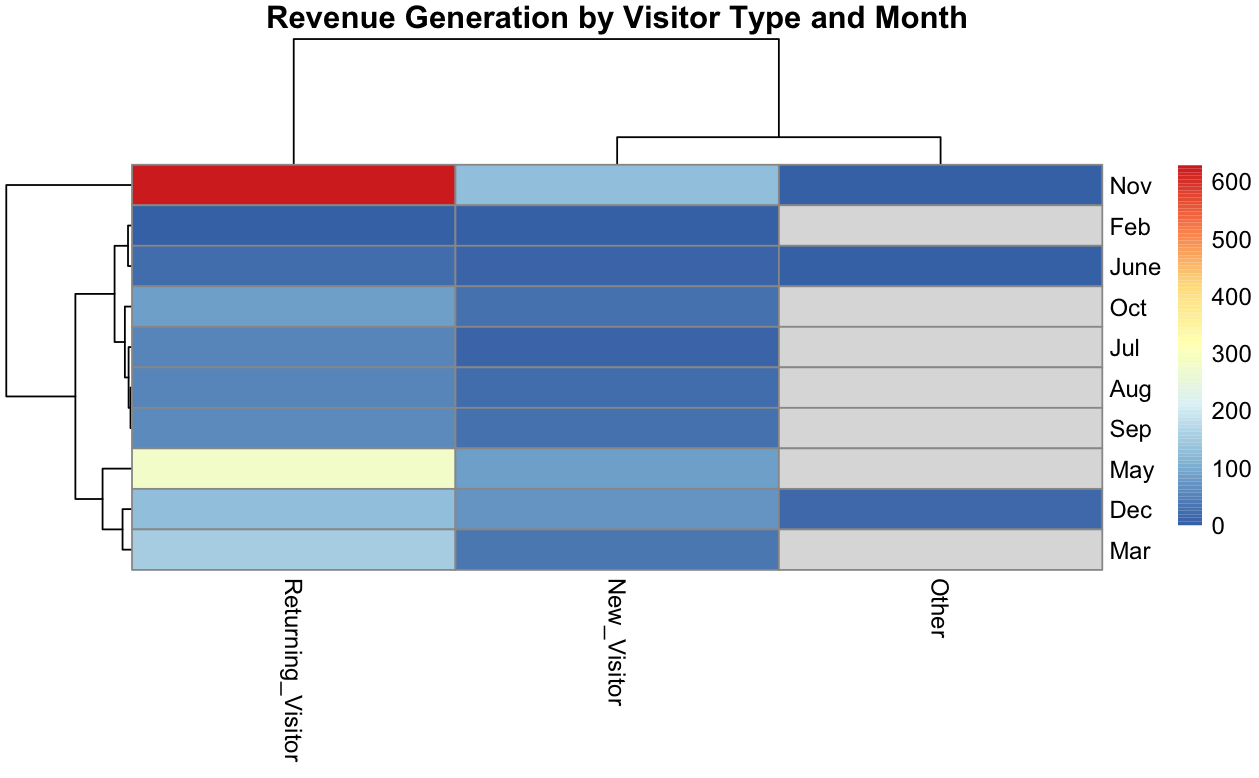
\includegraphics[width=0.82\textwidth]{Revenue Generation by Visitor Type and Month.png}  
    \caption{Revenue Generation by Visitor Type and Month}
\end{figure}
\vspace{0.5cm}

\textbf{Page Interaction and Revenue Optimization::}\\

\textbf{1. How do interactions between Product\-Related and Informational pages influence bounce rates and revenue generation? What improvements can be made to optimize the user experience and increase conversions through a balanced
focus on both types of content?} \\[5pt] % 

\FloatBarrier
Numerous important insights regarding user behavior and how it affects income production are provided by the scatter plot. First, as the teal-colored points suggest, consumers are more likely to make sales if they view a greater number of product-related pages. The red points, however, indicate that a sizable portion of customers also peruse numerous product pages without actually placing a purchase. This emphasizes the significance of the quality and relevancy of page content by implying that merely increasing the number of visits to the product page does not ensure conversions.


Users spend less time on informational pages on average, but those that interact with both product-related and informational pages in a moderate way are more likely to convert visitors into buyers. This implies that offering helpful, pertinent information in addition to product material can speed up decision-making and increase sales.


The relationship between income creation and bounce rates is also depicted in the figure. Bigger bubbles, which indicate higher bounce rates, are primarily linked to non-profitable consumers. On the other hand, buyers usually have reduced bounce rates. This emphasizes how crucial it is to maintain user engagement and lower the chance that users would depart the website too soon.


In conclusion, the results highlight the necessity of a well-rounded strategy that combines informational and product sites to engage users. Raising conversion rates and income can be achieved by enhancing the quality of both types of pages and reducing bounce rates.
\begin{figure}[h]
    \centering
    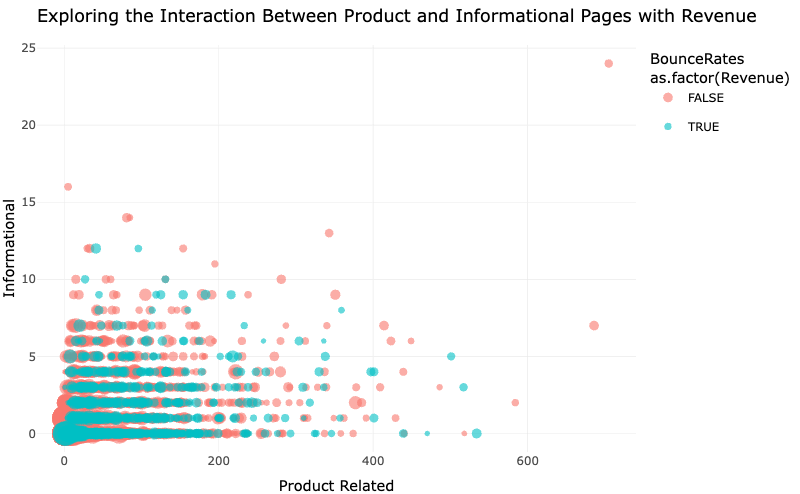
\includegraphics[width=0.82\textwidth]{Exploring the Interaction Between Product and Informational Pages with Revenue.png}  
    \caption{Exploring the Interaction Between Product and Informational Pages with Revenue}
\end{figure}
\vspace{0.5cm}
\newpage
























\section{Future Work}

In order to improve engagement and better tailor marketing techniques, future research could examine the demographic facets of user behavior, such as age, gender, and geography. Furthermore, studying how users behave on various device kinds (tablets, desktop computers, and mobile phones) may offer suggestions for improving the user interface on each platform. Examining how social media interactions, product recommendations, and customer reviews affect conversions may provide insightful information about improving user engagement and boosting revenue. Incorporating machine learning models to forecast consumer behavior and pinpoint possible discontinuity spots in the user journey has the potential to greatly enhance conversion rates and generate income.According to (FAWCETT & PROVOST, 2013), machine learning can be used to enhance predictive analytics by assisting in the identification of trends and deviations in consumer behavior, which can improve decision-making.

\section{Conclusion}

In order to determine the variables influencing income generation, we looked at important user behavior patterns on an e-commerce site. The study revealed that sales were mostly generated by returning visitors, underscoring the significance of customer retention. Conversely, new visitors had reduced conversion rates, indicating the necessity for enhanced engagement tactics. It was discovered that high rates of bounce and leave had a detrimental effect on income, suggesting that improving user experience and content could increase engagement.
Furthermore, conversions were primarily driven by a small number of traffic sources, indicating that companies should concentrate on optimizing their best-performing channels while simultaneously improving their least-effective ones. A significant factor in conversions was the interaction between product-related and informational pages, highlighting the need of well-written, well-balanced material. In summary, the report offers practical recommendations for enhancing user engagement, revenue creation, and conversions. To improve marketing and engagement tactics, future studies should look at demographic variables and device kinds.

\section{References}
\bibitem{Chaffey}
 Chaffey, D. and Ellis-Chadwick, F. (2022) Digital Marketing: Strategy, implementation and practice. Harlow: Pearson. 
 \bibitem{Xia}
  Xia, Y., Sun, J. and Chen, D.-G. (2018) ‘Introduction to R, rstudio and GGPLOT2’, ICSA Book Series in Statistics, pp. 77–127. doi:10.1007/978-981-13-1534-3_4.
  
  \bibitem{Islam}
  Islam, M. and Jin, S. (2019) ‘An overview of data visualization’, 2019 International Conference on Information Science and Communications Technologies (ICISCT) [Preprint]. doi:10.1109/icisct47635.2019.9012031.
  \bibitem{Wickham}
  Wickham, H. (2016) ‘GGPLOT2’, Use R! [Preprint]. doi:10.1007/978-3-319-24277-4. 
  
 
 


 
  


 

 \FloatBarrier


\FloatBarrier
FAWCETT, T. and PROVOST, F. (2013) Data Science for Business: What you need to know about data mining and data-analytic thinking Foster Provost, Tom Fawcett. Beijing ; Cambridge ; Farnham etc.: O’Reilly. 

\end{document}